\documentclass[11 pt,t]{beamer}
\usetheme[
	bullet=circle,		% Other option: square
	bigpagenumber,		% circled page number on lower right
	topline=true,		% colored bar at the top of the frame 
	]{Zurich}
\usepackage[utf8]{inputenc} % Required for inputting international characters


%-----------------------------------------------------------------------------
% DOCUMENT PROPERTIES

\author{\emph{author:}\\
Oriol \textsc{Colomés Gené}\\[0.2cm]
\emph{supervisor:}\\
Santiago \textsc{Badia}}
\title{Large scale Finite Element solvers for the large eddy simulation of incompressible turbulent flows}
\institute{Departament d'Enginyeria Civil i Ambiental}
\titlegraphic{
\includegraphics[width=0.3\textwidth]{../../sources/Figures/Cover/logo_escola_pantone_201_C}}
%\titlegraphic{
\includegraphics[width=0.7\texwidth]{../../sources/Figures/Cover/logo_escola_pantone_201_C.png}}

%-----------------------------------------------------------------------------


\begin{document}

%=========================================================================================
% TITLE
% ----------------------------------------------------------------------------
\addtocounter{framenumber}{-1}
\frame{\titlepage}
% ----------------------------------------------------------------------------

%=========================================================================================
% 1.MOTIVATION
% ----------------------------------------------------------------------------
\section{Motivation}

%=========================================================================================
% 2.RESIDUAL-BASED VMS
% ----------------------------------------------------------------------------
\section{Residual-based VMS}

%=========================================================================================
% 2.1.FORMULATION
% ----------------------------------------------------------------------------
\subsection{Formulation}

%=========================================================================================
% 2.2.ENERGY STATEMENTS
% ----------------------------------------------------------------------------
\subsection{Energy statements}

%=========================================================================================
% 2.3.NUMERICAL EXPERIMENTS
% ----------------------------------------------------------------------------
\subsection{Numerical experiments}

%=========================================================================================
% 2.3.1.DHIT
% ----------------------------------------------------------------------------
\subsubsection{DHIT}

%=========================================================================================
% 2.3.2.TGV
% ----------------------------------------------------------------------------


%=========================================================================================
% 2.3.3.TCF
% ----------------------------------------------------------------------------

%=========================================================================================
% 2.4.CONCLUSIONS
% ----------------------------------------------------------------------------

%=========================================================================================
% 3.MIXED FE VMS
% ----------------------------------------------------------------------------

%=========================================================================================
% 3.1.FORMULATION
% ----------------------------------------------------------------------------

%=========================================================================================
% 3.2.BLOCK-PRECONDITIONING
% ----------------------------------------------------------------------------

%=========================================================================================
% 3.3.NUMERICAL EXPERIMENTS
% ----------------------------------------------------------------------------

%=========================================================================================
% 3.3.1.TGV
% ----------------------------------------------------------------------------

%=========================================================================================
% 3.3.2.TCF
% ----------------------------------------------------------------------------

%=========================================================================================
% 3.4.CONCLUSIONS
% ----------------------------------------------------------------------------

%=========================================================================================
% 4.SRK
% ----------------------------------------------------------------------------

%=========================================================================================
% 4.1.FORMULATION
% ----------------------------------------------------------------------------

%=========================================================================================
% 4.2.NUMERICAL EXPERIMENTS
% ----------------------------------------------------------------------------

%=========================================================================================
% 4.2.1.ANALYTICAL
% ----------------------------------------------------------------------------

%=========================================================================================
% 4.2.2.CYLINDER
% ----------------------------------------------------------------------------

%=========================================================================================
% 4.3.CONCLUSIONS
% ----------------------------------------------------------------------------

%=========================================================================================
% 5.SVMS
% ----------------------------------------------------------------------------

%=========================================================================================
% 5.1.FORMULATION
% ----------------------------------------------------------------------------

%=========================================================================================
% 5.2.BLOCK-PRECONDITIONING
% ----------------------------------------------------------------------------

%=========================================================================================
% 5.3.NUMERICAL EXPERIMENTS
% ----------------------------------------------------------------------------

%=========================================================================================
% 5.3.1.TGV
% ----------------------------------------------------------------------------

%=========================================================================================
% 5.3.2.TCF
% ----------------------------------------------------------------------------

%=========================================================================================
% 5.3.3.NACA
% ----------------------------------------------------------------------------

%=========================================================================================
% 5.4.CONCLUSIONS
% ----------------------------------------------------------------------------

%=========================================================================================
% 6.CONCLUSIONS
% ----------------------------------------------------------------------------



\begin{frame}
\frametitle{Outline}
%\framesubtitle{Handwriting}

\begin{itemize}
    \item Line 1.
    \only<2->{
    \item Line 2.\\
        {\handwriting \textcolor{tangocolordarkchameleon}{Less formal} }
    }
    \only<3->{
    \item Line 3.\\
        {\handwriting \textcolor{tangocolordarkscarletred}{
        Less formal, different color.} }
    }
\end{itemize}


\end{frame}
% ----------------------------------------------------------------------------


% ----------------------------------------------------------------------------
\begin{frame}
\frametitle{Blocks}

\begin{block}{Standard Block}
    This is a standard block.
\end{block}

\begin{exampleblock}{Example Block}
    This is an example block.
\end{exampleblock}

\begin{alertblock}{Alert Block}
    This is an alert block.
\end{alertblock}



\end{frame}
% ----------------------------------------------------------------------------


% ----------------------------------------------------------------------------
\usebackgroundtemplate{
   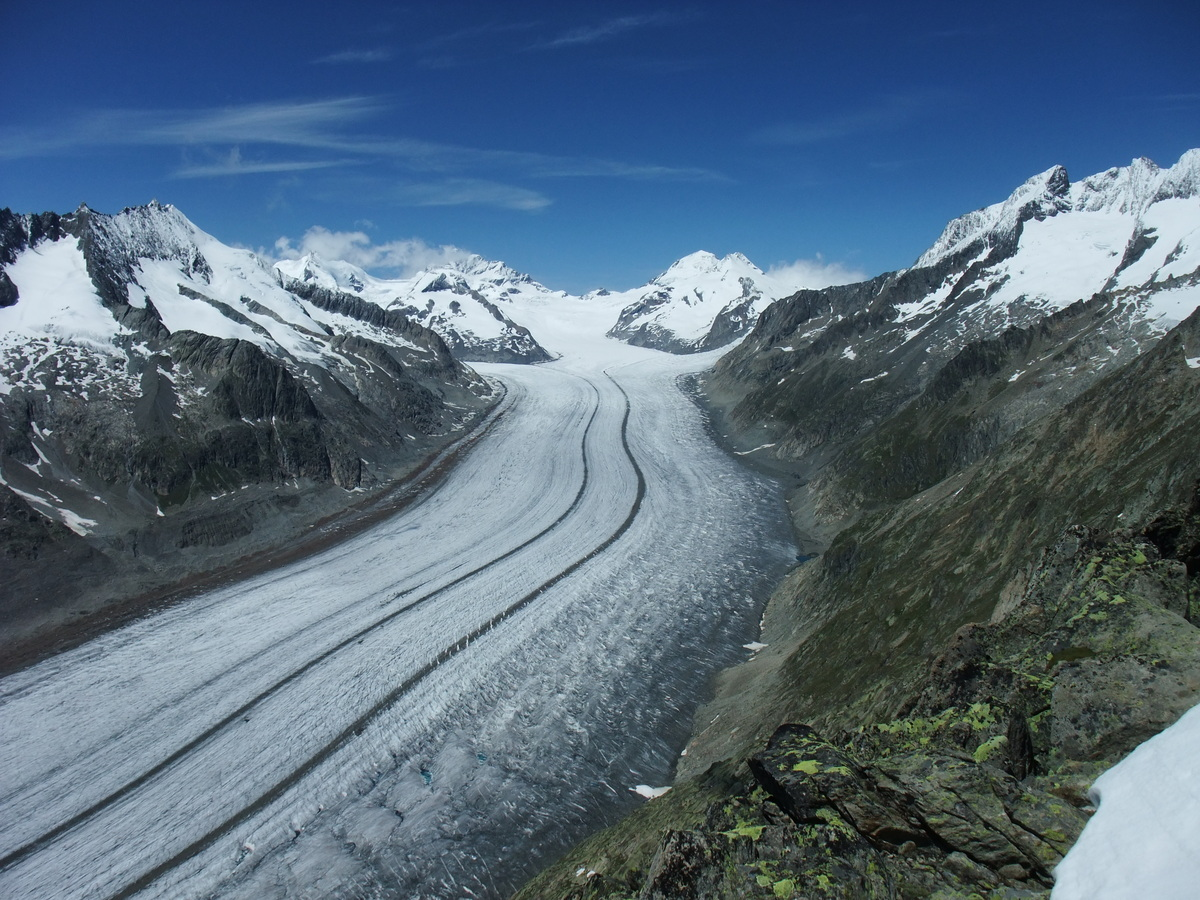
\includegraphics[width=\paperwidth,
                    height=\paperheight]{aletsch}
}
\begin{frame}
\ \\ \ \\
\centering \Large \textcolor{white}{Questions?}

\end{frame}
\usebackgroundtemplate{}
% ----------------------------------------------------------------------------


\end{document}
